\documentclass[12pt,a4paper]{article}

\usepackage[utf8]{inputenc}
\usepackage[T1]{fontenc}
\usepackage[french]{babel}

\usepackage{styles/couleurs}
\usepackage{styles/mise_en_page}
\usepackage{styles/boites}
\usepackage{styles/maths}
\usepackage{styles/figures}

\usepackage{amsmath}
\usepackage{amssymb}
\usepackage{enumitem}
\usepackage{graphicx}
\usepackage[most]{tcolorbox}
\usepackage{tikz}

\setlength{\parindent}{0pt}
\setlength{\parskip}{0pt}
\flushbottom

% =========================================================
% ESPACEMENTS
% =========================================================

\setlength{\abovedisplayskip}{3pt}
\setlength{\belowdisplayskip}{3pt}
\setlength{\abovedisplayshortskip}{2pt}
\setlength{\belowdisplayshortskip}{2pt}

\setlist[itemize]{
  leftmargin=1.3em,
  itemsep=0em,
  topsep=0.1em,
  parsep=0pt
}

% =========================================================
% COMMANDES
% =========================================================

\newcommand{\titresequence}[1]{%
\begin{center}
  {\sffamily\LARGE\bfseries\color{TitreC}
  Séquence 2 -- Théorème de Pythagore}\\[-0.05em]
  {\sffamily\large\bfseries\color{SavoirC}
  #1}
\end{center}
\vspace{-0.35em}
}

\newcommand{\minititre}[1]{%
{\sffamily\large\bfseries\color{SavoirC}#1}\par
\vspace{0.12em}
}

\newcommand{\touche}[1]{%
\fbox{%
  \rule{0pt}{1.15em}%
  \sffamily\bfseries\scriptsize #1%
}%
}

\begin{document}

% =========================================================
% PAGE 1
% =========================================================

\titresequence{Cours}

% =========================================================
\section{Rappel : le carré d'un nombre}
% =========================================================

\definition{
Le carré d'un nombre \(c\) est le produit de ce nombre par lui-même :

\[
\boxed{c^2=c\times c}
\]

Par exemple :
\[
5^2=25
\qquad\text{et}\qquad
3^2=9.
\]
}

Si un carré a pour côté \(c\), alors son aire est \(c^2\).

\vfill

% =========================================================
\section{L'hypoténuse}
% =========================================================

\definition{
Dans un triangle rectangle, le côté situé
\textbf{en face de l'angle droit}
s'appelle l'\textbf{hypoténuse}.
}

\begin{tcolorbox}[
  enhanced,
  colback=SavoirBg,
  colframe=SavoirC!45,
  boxrule=0.5pt,
  arc=1.5mm,
  left=3mm,
  right=3mm,
  top=0.8mm,
  bottom=0.8mm,
  before skip=1mm,
  after skip=1mm
]
\textbf{Propriété :}
l'hypoténuse est le \textbf{plus long côté} d'un triangle rectangle.
\end{tcolorbox}

Dans le triangle \(ABC\) rectangle en \(A\),
l'hypoténuse est \([BC]\).

\vfill

% =========================================================
\section{Du puzzle au théorème}
% =========================================================

\begin{minipage}[c]{0.35\linewidth}
\centering

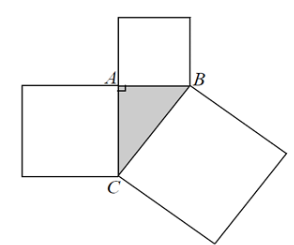
\includegraphics[
  width=0.92\linewidth,
  height=4.4cm,
  keepaspectratio
]{images/puzzle_original_triangle_carrés.png}

\end{minipage}
\hfill
\begin{minipage}[c]{0.61\linewidth}

Le puzzle montre que :

\[
\boxed{
\begin{array}{c}
\text{aire du carré sur l'hypoténuse}\\
=\\[-0.2em]
\text{somme des aires des deux autres carrés}
\end{array}
}
\]

Dans le triangle \(ABC\) rectangle en \(A\) :

\[
BC^2=AB^2+AC^2.
\]

\end{minipage}

\vfill

\theoreme{
Dans un triangle rectangle,
le carré de la longueur de l'hypoténuse
est égal à la somme des carrés des longueurs
des deux autres côtés.
}

\begin{center}
Si \(ABC\) est rectangle en \(A\), alors :
\[
\boxed{BC^2=AB^2+AC^2}
\]
\end{center}

% =========================================================
% PAGE 2
% =========================================================

\newpage
\small

% =========================================================
% RACINE CARRÉE
% =========================================================

\minititre{La racine carrée}

Lors de l'activité, nous avons cherché le côté d'un carré
d'aire \(50\ \text{cm}^2\) :

\[
7{,}07\times7{,}07=49{,}9849
\qquad
7{,}08\times7{,}08=50{,}1264.
\]

\vfill

% =========================================================
% SCHÉMATISATION
% =========================================================

\begin{tcolorbox}[
  enhanced,
  colback=white,
  colframe=SavoirC!45,
  boxrule=0.6pt,
  arc=1.5mm,
  left=4mm,
  right=4mm,
  top=1.5mm,
  bottom=1.5mm
]

\begin{center}
{\sffamily\bfseries\color{SavoirC}
Carré d'un nombre et racine carrée}
\end{center}

\noindent
\begin{minipage}[c]{0.46\linewidth}
\centering

{\sffamily\bfseries Du côté vers l'aire}

\vspace{0.2em}

\begin{tikzpicture}[scale=0.68]
\draw[thick] (0,0) rectangle (2.5,2.5);
\node at (1.25,1.25) {\large \(36\ \text{cm}^2\)};
\node[below] at (1.25,0) {\small \(6\ \text{cm}\)};
\end{tikzpicture}

\[
6\times6=36
\qquad
\boxed{6^2=36}
\]

\[
\boxed{
\text{côté}
\ \xrightarrow{\quad\text{carré}\quad}\
\text{aire}
}
\]

\end{minipage}
\hfill
\begin{minipage}[c]{0.46\linewidth}
\centering

{\sffamily\bfseries De l'aire vers le côté}

\vspace{0.2em}

\begin{tikzpicture}[scale=0.68]
\draw[thick] (0,0) rectangle (2.5,2.5);
\node at (1.25,1.25) {\large \(36\ \text{cm}^2\)};
\node[below] at (1.25,0) {\small côté \(=?\)};
\end{tikzpicture}

\[
\sqrt{36}=6
\qquad
\boxed{\text{côté}=6\text{ cm}}
\]

\[
\boxed{
\text{aire}
\ \xrightarrow{\quad\text{racine carrée}\quad}\
\text{côté}
}
\]

\end{minipage}

\end{tcolorbox}

\vfill

% =========================================================
% DÉFINITION
% =========================================================

\definition{
La \textbf{racine carrée} d'un nombre positif \(a\)
est le nombre positif dont le carré est égal à \(a\).

\[
\boxed{\sqrt{a}}
\qquad
\sqrt{49}=7
\qquad
\sqrt{81}=9
\qquad
\sqrt{50}\approx7{,}07
\]
}

\vfill

% =========================================================
% CALCULATRICE
% =========================================================

\minititre{Avec la calculatrice}

\noindent
\begin{minipage}[t]{0.485\textwidth}
\vspace{0pt}

\begin{tcolorbox}[
  enhanced,
  colback=SavoirBg,
  colframe=SavoirC!45,
  boxrule=0.5pt,
  arc=1.5mm,
  left=2.5mm,
  right=2.5mm,
  top=1mm,
  bottom=1mm
]

{\sffamily\bfseries\color{SavoirC}
CASIO fx-92+ Spéciale Collège}

\[
\sqrt{50} :
\quad
\touche{SECONDE}\;
\touche{\(x^2\)}\;
\touche{50}\;
\touche{EXE}
\]

\[
\touche{\(S\leftrightarrow D\)}
\quad\Rightarrow\quad
\boxed{\sqrt{50}\approx7{,}07}
\]

\end{tcolorbox}

\end{minipage}
\hfill
%
\begin{minipage}[t]{0.485\textwidth}
\vspace{0pt}

\begin{tcolorbox}[
  enhanced,
  colback=SavoirBg,
  colframe=SavoirC!45,
  boxrule=0.5pt,
  arc=1.5mm,
  left=2.5mm,
  right=2.5mm,
  top=1mm,
  bottom=1mm
]

{\sffamily\bfseries\color{SavoirC}
Nouvelle CASIO fx-92 Collège}

{\scriptsize Modèle à touches rondes}

\[
\sqrt{50} :
\quad
\touche{\(\sqrt{\phantom{0}}\)}\;
\touche{50}\;
\touche{EXE}
\]

\[
\touche{FORMAT}
\rightarrow
\touche{Décimal}
\quad\Rightarrow\quad
\boxed{\sqrt{50}\approx7{,}07}
\]

\end{tcolorbox}

\end{minipage}

% =========================================================
% PAGE 3
% =========================================================

\newpage
\small

% =========================================================
% ARRONDI
% =========================================================

\minititre{Arrondir au dixième}

\begin{tcolorbox}[
  enhanced,
  colback=SavoirBg,
  colframe=SavoirC!45,
  boxrule=0.5pt,
  arc=1.5mm,
  left=4mm,
  right=4mm,
  top=1.5mm,
  bottom=1.5mm
]

Pour arrondir au dixième, je garde \textbf{un chiffre après la virgule}
et je regarde le \textbf{chiffre suivant} :

\[
\boxed{
\begin{array}{ccl}
0,\ 1,\ 2,\ 3,\ 4 &\longrightarrow& \text{je garde le dixième}\\[0.2em]
5,\ 6,\ 7,\ 8,\ 9 &\longrightarrow& \text{j'ajoute 1 au dixième}
\end{array}
}
\]

\[
\sqrt{50}\approx7{,}\boxed{0}\underline{7}\ldots
\quad\Longrightarrow\quad
\boxed{\sqrt{50}\approx7{,}1}
\]

\[
\sqrt{55}\approx7{,}\boxed{4}\underline{1}\ldots
\quad\Longrightarrow\quad
\boxed{\sqrt{55}\approx7{,}4}
\]

\begin{center}
Un arrondi n'est pas exact :
\[
\boxed{\sqrt{50}\approx7{,}1}
\qquad\text{et non}\qquad
\sqrt{50}=7{,}1.
\]
\end{center}

\end{tcolorbox}

\vspace{0.4em}

% =========================================================
% RÉDIGER
% =========================================================

\minititre{Rédiger avec le théorème de Pythagore}

\noindent
\begin{minipage}[t]{0.485\textwidth}
\vspace{0pt}

\begin{tcolorbox}[
  enhanced,
  colback=white,
  colframe=ActionC!55,
  boxrule=0.6pt,
  arc=2mm,
  left=3mm,
  right=3mm,
  top=1.5mm,
  bottom=1.5mm
]

{\sffamily\bfseries\color{ActionC}
Chercher l'hypoténuse}

\smallskip

\(MNP\) est rectangle en \(M\), avec
\(MN=5\) cm et \(MP=7\) cm.

Calculer \(NP\).

\smallskip

\textbf{Rédaction}

\smallskip

Le triangle \(MNP\) est rectangle en \(M\).

D'après le théorème de Pythagore :

\[
NP^2=MN^2+MP^2
\]

\[
\begin{aligned}
NP^2 &= 5^2+7^2\\
NP^2 &= 25+49\\
NP^2 &= 74
\end{aligned}
\]

\[
NP=\sqrt{74}
\]

\[
\boxed{NP\approx8{,}6\text{ cm}}
\]

\end{tcolorbox}

\end{minipage}
\hfill
%
\begin{minipage}[t]{0.485\textwidth}
\vspace{0pt}

\begin{tcolorbox}[
  enhanced,
  colback=white,
  colframe=ActionC!55,
  boxrule=0.6pt,
  arc=2mm,
  left=3mm,
  right=3mm,
  top=1.5mm,
  bottom=1.5mm
]

{\sffamily\bfseries\color{ActionC}
Chercher un côté de l'angle droit}

\smallskip

\(RST\) est rectangle en \(R\), avec
\(ST=9\) cm et \(RS=4\) cm.

Calculer \(RT\).

\smallskip

\textbf{Rédaction}

\smallskip

Le triangle \(RST\) est rectangle en \(R\).

D'après le théorème de Pythagore :

\[
ST^2=RS^2+RT^2
\]

\[
\begin{aligned}
9^2 &= 4^2+RT^2\\
81 &= 16+RT^2\\
RT^2 &= 81-16\\
RT^2 &= 65
\end{aligned}
\]

\[
RT=\sqrt{65}
\]

\[
\boxed{RT\approx8{,}1\text{ cm}}
\]

\end{tcolorbox}

\end{minipage}

\vspace{0.3em}

% =========================================================
% CHECKLIST
% =========================================================

\minititre{Ma checklist Pythagore}

\begin{tcolorbox}[
  enhanced,
  colback=ActionC!5,
  colframe=ActionC!55,
  boxrule=0.6pt,
  arc=2mm,
  left=4mm,
  right=4mm,
  top=1.2mm,
  bottom=1.2mm
]

\begin{minipage}[t]{0.48\linewidth}

\(\square\) Le triangle est \textbf{rectangle}.

\smallskip

\(\square\) J'ai repéré l'\textbf{hypoténuse}.

\smallskip

\(\square\) L'hypoténuse est seule d'un côté de l'égalité.

\smallskip

\(\square\) J'écris d'abord l'égalité avec les \textbf{lettres}.

\end{minipage}
\hfill
\begin{minipage}[t]{0.48\linewidth}

\(\square\) Je prends la \textbf{racine carrée}.

\smallskip

\(\square\) Si j'arrondis, j'écris \(\approx\).

\smallskip

\(\square\) J'écris l'\textbf{unité}.

\smallskip

\(\square\) Je vérifie : l'hypoténuse est le \textbf{plus long côté}.

\end{minipage}

\end{tcolorbox}

\end{document}